\chapter{Cài đặt}

\section{Yêu cầu và chức năng của hệ thống}

Yêu cầu hệ thống tìm kiếm:
\begin{itemize}
    \item Hỗ trợ tìm kiếm theo chức năng thông thường và tìm kiếm theo ngữ nghĩa.
    \item Có một ontology mô tả tri thức lĩnh vực sách CNTT.
    \item Kết quả đáp ứng được nhu cầu tìm kiếm của người dùng.
\end{itemize}

Hệ thống cho phép tìm kiếm theo các cách thức sau:
\begin{enumerate}
    \item Tìm kiếm so trùng dựa vào mọi từ người dùng nhập vào. Kết quả trả về bao gồm tài liệu có các thành phần sau chứa từ khóa tìm kiếm: tiêu đề sách, tên tác giả, tập từ khóa tài liệu.
    \item Tìm kiếm không so trùng chính xác tuyệt đối từ khóa người dùng nhập vào. Hệ thống sẽ tách câu, tách từ, chọn lọc bổ sung các từ khóa sử dụng ontology. Sau đó dùng các từ khóa này để so trùng như cách 1.
\end{enumerate}


\section{Kiến trúc hệ thống}
Kiến trúc hệ thống như sau:

\begin{figure}[H]
    \centering
    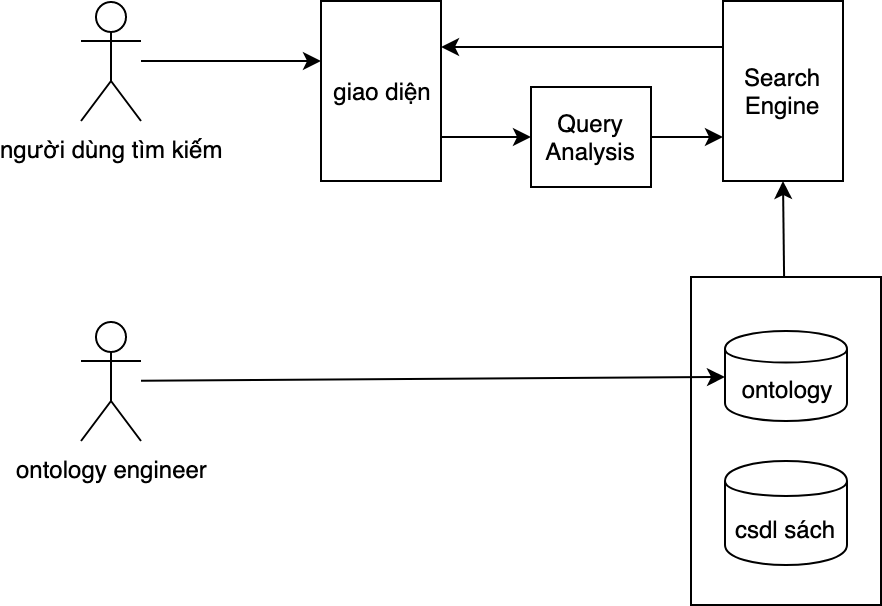
\includegraphics[width=0.8\textwidth]{img/sys_design.png}
    \caption{Kiến trúc hệ thống tìm kiếm ngữ nghĩa với Ontology}
\end{figure}

Mô tả các thành phần trong hệ thống:
\begin{itemize}
    \item \textbf{Database}: cơ sở dữ liệu của toàn hệ thống bao gồm \textit{CSDL SACH} lưu trữ thông tin sách cho hệ thống và \textit{CSDL ONTOLOGY} là ontology cho sách lĩnh vực CNTT.
    \item \textbf{Giao diện}: giao tiếp giữa người dùng và hệ thống.
    \item \textbf{Query Analysis}: tiếp nhận thông tin từ \textbf{Giao diện} chuẩn hóa thông tin sau đó đưa thông tin đến \textbf{Search Engine} của hệ thống.
    \item \textbf{Search Engine}: bộ tìm kiếm sẽ nhận thông tin theo cấu trúc đặc tả từ Query Analysis sau đó thực hiện tìm kiếm, trả kết quả về Giao diện.
    
\end{itemize}

\section{Cài đặt}

Các bước cài đặt bao gồm:
\begin{itemize}
    \item Xây dựng Ontology cho ứng dụng.
    \item Xây dựng thành phần tạo chỉ mục.
    \item Xây dựng thành phần xử lý câu truy vấn và truy vấn dữ liệu dựa trên yêu cầu truy vấn người dùng.
\end{itemize}

\subsection{Xây dựng Ontology}
Các khái niệm được sử dụng trong cơ sở tri thức Ebook là những khái niệm thuộc lĩnh vực giáo dục, được trính ra từ các sách thu thập được trên hệ thống. Báo cáo chỉ tập trung phục vụ tra cứu cho một nhóm nhỏ sách ebook thuộc lĩnh vực CNTT, nên sẽ xây dựng ontology dựa trên dữ liệu sách này.

Ontology trong báo cáo này được rút trích từ mục lục các quyển sách phổ biến trên hệ thống. Các công việc bao gồm thực hiện việc phân loại và rút trích keyphrase từ mục lục, công việc được thực hiện một cách thủ công.

\subsubsection{Thiết kế lớp}
Từ các dữ liệu thu thập được, đề tài đưa ra 7 lớp như sau:
\begin{enumerate}
    \item \textit{TacGia}: lớp tổng quan về tác giả.
    \item \textit{Sach}: lớp tổng quan về sách.
    \item \textit{Keyphrase}: lớp tổng quan về Keyphrase. Gồm các lớp con sau:
    \item \textit{CNTT}: lớp các keyphrase về sách chuyên ngành công nghệ thông tin.
    \item \textit{ML}: lớp các keyphrase về sách chuyên ngành trí tuệ nhân tạo Machine Learning.
    \item \textit{ThietKeWeb}: lớp các keyphrase về sách thiết kế Website.
    \item \textit{CSDL}: lớp các keyphrase về sách cơ sở dữ liệu.
\end{enumerate}

\subsubsection{Thuộc tính lớp}
Các thuộc tính lớp được xây dựng cho ứng dụng dựa trên chuẩn từ vựng Dublin Core và được bổ sung thêm:


\begin{itemize}
    \item\textit{ma\_sach}: mã sách trên hệ thống.
    \item\textit{tieu\_de}: tiêu đề sách ebook.
    \item\textit{ten\_tg}: tiêu tác giả.
    \item\textit{key\_phrase}: danh sách keyphrase biểu diễu nội dung sách.
\end{itemize}


\subsubsection{Các mối quan hệ}
Xây dựng các mối quan hệ bao gồm:

\begin{itemize}
    \item Quan hệ liên quan giữa các lớp:
    \begin{itemize}
        \item Quan hệ giữa Sách và Tác giả: Sach \textbf{coTacGia} TacGia
        \item Quan hệ giữa Tác giả và Sách: TacGia \textbf{laTacGiaCua} Sach
        \item Quan hệ giữa Sách và Tác Giả Phụ: TacGia \textbf{coTacGiaPhu} Sach
        \item Quan hệ giữa Sách và Keyphrase: Sach \textbf{coKeyphrase} Keyphrase
        \item Quan hệ giữa Keyphrase và Sách: Keyphrase \textbf{coKeyphrase} Sach. 
    \end{itemize}
    
    \item Quan hệ giữa các keyphrase:
    \begin{itemize}
        \item Quan hệ đồng nghĩa
        \item Quan hệ viết tắt
        \item Quan hệ cùng lớp  
    \end{itemize}
    
    \item Quan hệ phân cấp trên lớp
    
    \begin{figure}[H]
        \centering
        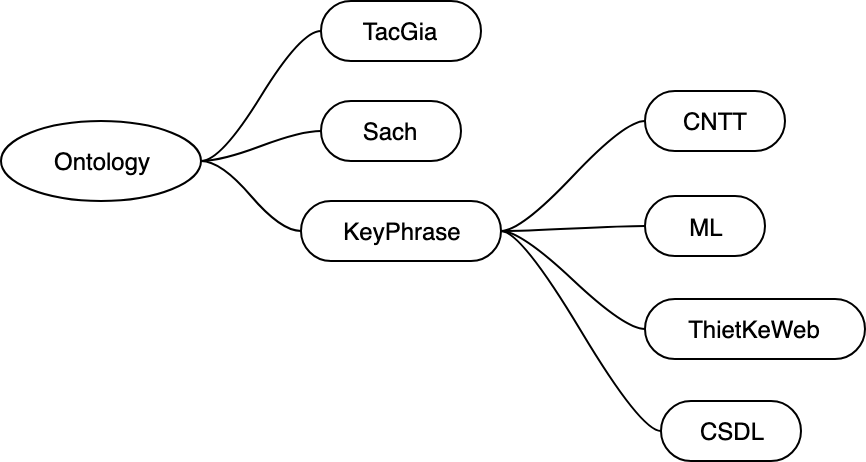
\includegraphics[width=0.8\textwidth]{img/cay_phan_cap.png}
        \caption{Minh họa các quan hệ phân cấp trên lớp}
        \label{fig:quan_he_phan_cap}
    \end{figure}
    
    % Bảng mô tả các lớp:
    
    
\end{itemize}



\subsection{Xây dựng các thành phần tạo chỉ mục}
Thành phần tạo chỉ mục bao gồm các chức năng chính như chỉ định dữ liệu lập chỉ mục, thực hiện phân tích tài liệu, tạo chỉ mục và lưu trữ. Thành phần này kế thừa từ thư viện Apache Solr và Lucene. 

\subsection{Xây dựng thành phần truy vấn}

Thành phần truy vấn gồm các chức năng chính như: nhận thông tin truy vấn, chuyển đổi từ truy vấn và tìm kiếm, hiển thị kết quả trả về. Thành phần biên dịch truy vấn và tìm kiếm cũng kế thừa từ Apache Solr. Quy trình tổng quát như hình \ref{fig:mo_hinh_tim_kiem}.


   \begin{figure}[H]
        \centering
        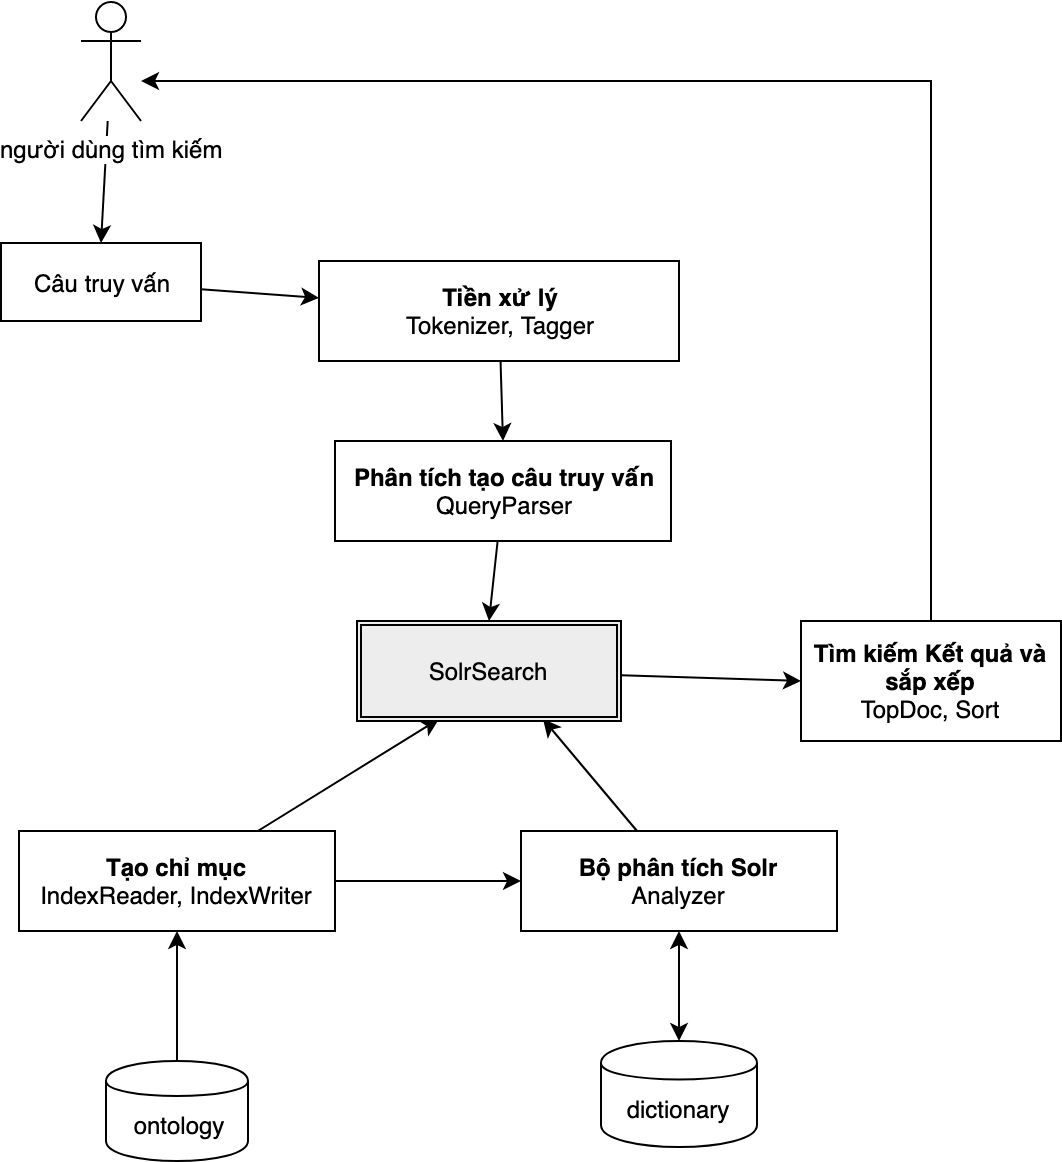
\includegraphics[width=0.8\textwidth]{img/so_do_he_thong.png}
        \caption{Quy trình xử lý trên hệ thống tìm kiếm}
        \label{fig:mo_hinh_tim_kiem}
    \end{figure}
    
    
\begin{itemize}
    \item \textbf{Chuẩn bị dữ liệu cho hệ thống tìm kiếm thực hiện qua các bước}
    \begin{enumerate}
        \item Đọc file ontology
        \item Tạo cây dữ liệu từ ontology: \textit{CreateNodes}
        \item Tạo chi mục tìm kiếm: \textit{IndexReader, IndexWriter}
    \end{enumerate}
    
    \item \textbf{Quy trình xử lý tìm kiếm hiện qua các bước}
    \begin{enumerate}
        \item Người dùng nhập câu
        \item Tiền xử lý: tách từ, gán nhãn cho câu truy vấn
        \item Xây dựng cây truy vấn theo chuẩn Apache Solr: \textit{QueryParser}
        \item Thực hiện tìm kiếm: \textit{SolrSearch}
        \item Đánh giá kết quả và sắp xếp theo độ đo: \textit{TopDoc, TopDoc.Sort}
        \item Hiển thị kết quả cho người dùng.
    \end{enumerate}
    
    
    \item \textbf{Thuật toán}
    \begin{itemize}
        \item Thuật toán xây dựng cấu trúc tìm kiếm từ file Ontology
        
        \begin{lstlisting}[language=Python,numbers=left,frame=single, basicstyle=\ttfamily\small]
loadOntology(iw IndexWriter, o Sach):
    iw.MaSach = getMaSach(s)
    iw.TuaSach = getTuaSach(s)
    
    while KeyPhrase in getKeyPhrase(s):
        iw.KeyPhase[] = KeyPhrase
        
    while TacGia in getTacGia(s):
        iw.TacGia[] = TacGia
        \end{lstlisting}

    \item Lấy toàn bộ thông tin sách và load vào Solr Index

 \begin{lstlisting}[language=Python,numbers=left,frame=single, basicstyle=\ttfamily\small]
buildIndex():
    // Khoi tao IndexWriter
    IndexWrite iw = IndexWrite{}
    
    // Lay danh sach ebooks tu Database
    Sach[] books = getBooksFromDB()
    
    // Load vao index Solr
    while book in books:
        loadOntology(iw, book)
        \end{lstlisting}

    \end{itemize}
    
    
    \item \textbf{Giao diện tìm kiếm Apache Solr}
    
    Hình \ref{fig:solr_client} thể hiện giao diện tìm kiếm của Apache Solr Client dưới dạng web, kết quả trả về có thể ở dạng JSON hoặc XML, dễ dàng tích hợp vào các hệ thống Web hoặc Application khác.
     
     \begin{figure}[H]
        \centering
        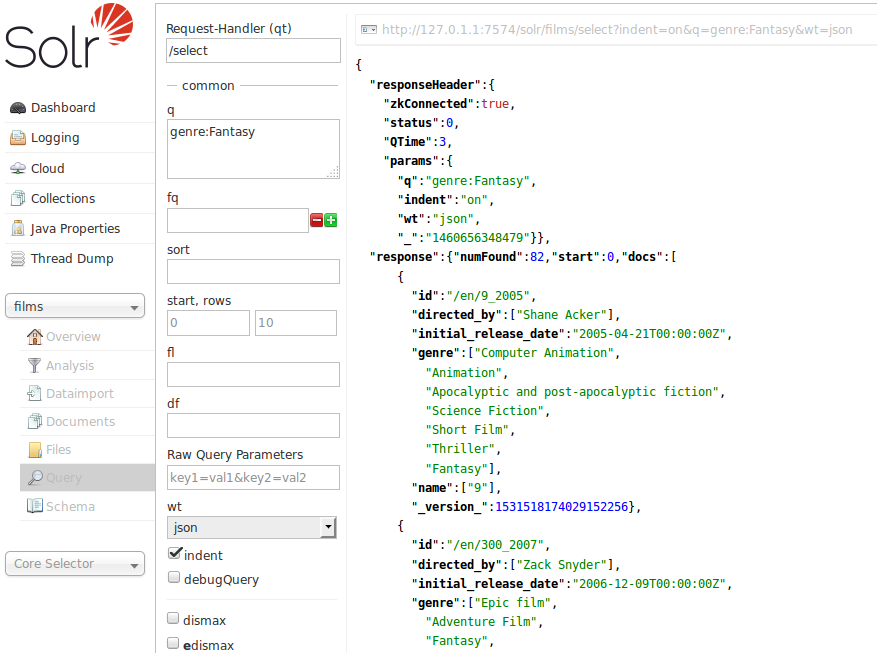
\includegraphics[width=1\textwidth]{img/solr.png}
        \caption{Giao diện tìm kiếm Apache Solr Client}
        \label{fig:solr_client}
    \end{figure}
    
    
\end{itemize}
